%% ============================================================
%%  Treehouse Ghana Instagram Intelligence Report
%%  Combined: Performance Overview · Engagement Analysis ·
%%            Advanced Statistical and Predictive Analysis
%%  Prepared by Odwira and Whitehall
%%  Author: Bernard Ashiley
%%  Date: 31 May 2026
%% ============================================================
\documentclass[11pt,a4paper]{report}

%% --- Packages -----------------------------------------------
\usepackage[a4paper, top=2.5cm, bottom=2.5cm,
            left=2.8cm, right=2.8cm]{geometry}
\usepackage[T1]{fontenc}
\usepackage[utf8]{inputenc}
\usepackage{lmodern}
\usepackage{microtype}
\usepackage{xcolor}
\usepackage{booktabs}
\usepackage{longtable}
\usepackage{array}
\usepackage{tabularx}
\usepackage{multirow}
\usepackage{parskip}
\usepackage{titlesec}
\usepackage{fancyhdr}
\usepackage{pgfplots}
\usepackage{tikz}
\usepackage{pgfplotstable}
\usepackage{hyperref}
\usepackage{enumitem}
\usepackage{caption}
\usepackage{mdframed}
\usepackage{graphicx}
\usepackage{amsmath}
\usepackage{pifont}
\pgfplotsset{compat=1.18}

%% --- Colour palette -----------------------------------------
\definecolor{tggreen}{HTML}{1B3A2D}
\definecolor{tgmid}{HTML}{2D6A4F}
\definecolor{tglight}{HTML}{D8F3DC}
\definecolor{tggold}{HTML}{C9A84C}
\definecolor{tgblue}{HTML}{2E86AB}
\definecolor{tgpurple}{HTML}{7B2D8B}
\definecolor{tggrey}{HTML}{4B5563}
\definecolor{tglightgrey}{HTML}{F3F4F6}
\definecolor{tgrule}{HTML}{D1D5DB}

%% --- Hyperref -----------------------------------------------
\hypersetup{
  colorlinks = true,
  linkcolor  = tggreen,
  urlcolor   = tgblue,
  citecolor  = tggreen,
  pdfauthor  = {Bernard Ashiley -- Odwira and Whitehall},
  pdftitle   = {Treehouse Ghana Instagram Intelligence Report},
  pdfsubject = {Public engagement, audience intent, and content strategy analysis}
}

%% --- Section formatting -------------------------------------
\titleformat{\chapter}[display]
  {\normalfont\Large\bfseries\color{tggreen}}
  {\chaptername\ \thechapter}{10pt}{\Huge}
\titleformat{\section}
  {\normalfont\large\bfseries\color{tggreen}}{}{0em}{}[\color{tgrule}\titlerule]
\titleformat{\subsection}
  {\normalfont\normalsize\bfseries\color{tgmid}}{}{0em}{}
\titleformat{\subsubsection}
  {\normalfont\normalsize\itshape\color{tggrey}}{}{0em}{}

%% --- Header / footer ----------------------------------------
\pagestyle{fancy}
\fancyhf{}
\fancyhead[L]{\small\color{tggrey}\textit{Treehouse Ghana Instagram Intelligence Report}}
\fancyhead[R]{\small\color{tggrey}\textit{Odwira and Whitehall --- Confidential}}
\fancyfoot[C]{\small\color{tggrey}\thepage}
\renewcommand{\headrulewidth}{0.4pt}
\renewcommand{\headrule}{\color{tgrule}\hrule width\headwidth height\headrulewidth}

%% --- Callout box --------------------------------------------
\newmdenv[
  linecolor=tggreen,
  backgroundcolor=tglight,
  linewidth=1pt,
  roundcorner=4pt,
  innerleftmargin=12pt,
  innerrightmargin=12pt,
  innertopmargin=10pt,
  innerbottommargin=10pt
]{callout}

\newmdenv[
  linecolor=tggold,
  backgroundcolor=tglightgrey,
  linewidth=1pt,
  roundcorner=4pt,
  innerleftmargin=12pt,
  innerrightmargin=12pt,
  innertopmargin=10pt,
  innerbottommargin=10pt
]{note}

%% --- Table column types -------------------------------------
\newcolumntype{L}[1]{>{\raggedright\arraybackslash}p{#1}}
\newcolumntype{R}[1]{>{\raggedleft\arraybackslash}p{#1}}
\newcolumntype{C}[1]{>{\centering\arraybackslash}p{#1}}

%% --- Caption setup ------------------------------------------
\captionsetup{font=small, labelfont={bf,color=tggreen},
              labelsep=period, skip=4pt}

%% ============================================================
\begin{document}

%% ============================================================
%%  COVER PAGE
%% ============================================================
\begin{titlepage}
  \pagecolor{tggreen}
  \color{white}
  \vspace*{3cm}
  \begin{center}
    {\fontsize{11}{13}\selectfont\textit{Odwira and Whitehall}}\\[6pt]
    {\color{tggold}\rule{6cm}{1pt}}\\[28pt]
    {\fontsize{34}{40}\selectfont\bfseries Treehouse Ghana}\\[10pt]
    {\fontsize{18}{24}\selectfont Instagram Intelligence Report}\\[18pt]
    {\color{tggold}\rule{10cm}{0.6pt}}\\[22pt]
    {\fontsize{12}{16}\selectfont
      Public engagement, audience intent, and content strategy analysis\\[4pt]
      Prepared from public Instagram data for Treehouse Ghana (\texttt{@treehousegh})}\\[40pt]
    {\fontsize{11}{14}\selectfont
      \textbf{Prepared by:} Bernard Ashiley\\[4pt]
      \textbf{Organisation:} Odwira and Whitehall\\[4pt]
      \textbf{Date:} 31 May 2026\\[4pt]
      \textbf{Classification:} Confidential}
  \end{center}
  \vfill
  \begin{center}
    {\small\color{white!70!tggreen}
      This document contains three integrated sections: a performance overview
      for operational stakeholders, a detailed engagement and content analysis,
      and a full advanced statistical and predictive analysis including
      Monte Carlo simulation results. No section has been abridged.}
  \end{center}
\end{titlepage}
\nopagecolor

%% ============================================================
\tableofcontents
\newpage

%% ============================================================
%%  PART I: PERFORMANCE OVERVIEW
%% ============================================================
\part{Performance Overview}

\chapter{At a Glance}

The following figures summarise the state of the public Instagram presence for Treehouse Ghana at the time of data collection. All metrics are derived entirely from public data; private account analytics (reach, impressions, saves, shares, profile visits, link clicks) are excluded and remain visible only within the native Instagram Insights dashboard.

\vspace{10pt}
\begin{callout}
\begin{tabularx}{\linewidth}{@{}L{4.2cm} X@{}}
  \textbf{Followers}           & 27,386 at time of collection \\[4pt]
  \textbf{Posts analysed}      & 135 owned feed posts and 84 short videos (reels) \\[4pt]
  \textbf{Top content category}& Cocktails and Drinks (average engagement score: 290) \\[4pt]
  \textbf{Best day to post}    & Monday (average engagement score: 199) \\[4pt]
  \textbf{Short video uplift}  & Short videos attracted 121\% more engagement than static posts on average \\
\end{tabularx}
\end{callout}

\vspace{10pt}
Treehouse Ghana holds a well-established Instagram presence. Short videos consistently outperform static posts. The principal opportunity identified in this analysis is an increase in drinks, events, and ambience content, paired with clearer calls to action in every caption.

\section{Data Coverage}

\begin{table}[h]
\centering
\caption{Summary of data collected for analysis}
\begin{tabular}{@{}L{7cm} R{4cm}@{}}
\toprule
\textbf{Area} & \textbf{Count} \\
\midrule
Owned feed posts analysed        & 135 \\
Reels analysed                   & 84  \\
Third-party mentions analysed    & 21  \\
Comments analysed                & 106 \\
Followers at collection time     & 27,386 \\
\bottomrule
\end{tabular}
\end{table}

Profile biography: \textit{Al fresco dining in the heart of Accra. Open daily from noon to 11pm.}

\begin{note}
\textbf{Data limitation.} This analysis covers public Instagram data only. It does not include private account analytics such as reach, impressions, saves, shares, profile visits, link clicks, story taps, ad spend, or completed bookings. All conclusions are directional rather than absolute. For business decisions, combine these findings with Treehouse Ghana's native Instagram analytics, reservation data, point-of-sale trends, and campaign context.
\end{note}

\chapter{Content Performance}

\section{Engagement Score Methodology}

The engagement score used throughout this report is calculated as follows:

\begin{equation*}
  \text{Engagement Score} = \text{Likes} + ({\text{Comments}} \times 5) + \left(\frac{\text{Views or Plays}}{100}\right)
\end{equation*}

This is not a replacement for native analytics. It is, however, a consistent and reproducible measure for comparing posts where only partial public metrics are available. Comments are weighted at five times the value of a like because they require active intent and carry greater commercial signal.

\section{What Content Performs Best}

The chart below ranks each content category by average engagement score across all posts in the dataset.

\vspace{8pt}
\begin{figure}[h]
\centering
\caption{Average engagement score by content pillar}
\begin{tikzpicture}
\begin{axis}[
  xbar, xmin=0, xmax=420,
  width=13.5cm, height=9.5cm,
  bar width=13pt,
  xlabel={\small Average engagement score},
  symbolic y coords={
    Reservations,
    Date Night,
    Birthdays,
    Price and Value,
    General Brand,
    Food,
    Promotions,
    Dinner and Nightlife,
    Ambience and Vibe,
    Events and Music,
    Cocktails and Drinks
  },
  ytick=data,
  y tick label style={font=\small, align=right, text width=3.8cm},
  nodes near coords,
  nodes near coords align={horizontal},
  every node near coord/.style={font=\footnotesize, color=tggreen},
  enlarge y limits=0.08,
  tick label style={font=\small},
  label style={font=\small},
  axis line style={draw=tgrule},
]
\addplot[fill=tgmid!80, draw=tgmid] coordinates {
  (35.54,  Reservations)
  (76.07,  Date Night)
  (76.73,  Birthdays)
  (79.84,  Price and Value)
  (80.36,  General Brand)
  (133.73, Food)
  (143.81, Promotions)
  (197.94, Dinner and Nightlife)
  (232.75, Ambience and Vibe)
  (251.93, Events and Music)
  (289.59, Cocktails and Drinks)
};
\end{axis}
\end{tikzpicture}
\end{figure}

\subsection{Top Five Content Categories}

\begin{enumerate}[leftmargin=*, label=\arabic{enumi}.]
  \item \textbf{Cocktails and Drinks} (average score: 290). Drinks content supports nightlife, after-work, and group-visit occasions. This category should receive increased investment.
  \item \textbf{Events and Live Music} (average score: 252). Event content must carry clear dates, artist names, set times, and booking instructions. Without these details, the post cannot convert interest to attendance.
  \item \textbf{Ambience and Vibe} (average score: 233). Venue-experience content sells the setting and should be paired with reservation details in every caption.
  \item \textbf{Dinner and Nightlife} (average score: 198). Evening content should highlight atmosphere, availability, and weekly programme rituals.
  \item \textbf{Promotions and Offers} (average score: 144). Offers should carry explicit expiry dates and a measurable response prompt, such as a WhatsApp number or a code.
\end{enumerate}

\section{Full Content Pillar Breakdown}

\begin{longtable}{@{}L{4cm} R{1.6cm} R{2cm} R{2cm} R{2cm} R{2.2cm}@{}}
\caption{Content pillar performance summary} \\
\toprule
\textbf{Pillar} & \textbf{Posts} & \textbf{Avg Likes} & \textbf{Avg Cmts} & \textbf{Avg Views} & \textbf{Avg Score} \\
\midrule
\endfirsthead
\multicolumn{6}{c}{\tablename\ \thetable{} --- continued} \\
\toprule
\textbf{Pillar} & \textbf{Posts} & \textbf{Avg Likes} & \textbf{Avg Cmts} & \textbf{Avg Views} & \textbf{Avg Score} \\
\midrule
\endhead
\bottomrule
\endfoot
\bottomrule
\endlastfoot
Cocktails and Drinks       & 11  & 132.00  & 2.91  & 14,304 & 289.59 \\
Events and Music      & 8   & 121.75  & 2.38  & 11,830 & 251.93 \\
Ambience and Vibe          & 15  & 123.07  & 14.20 & 3,869  & 232.75 \\
Dinner and Nightlife       & 17  & 86.71   & 2.06  & 10,094 & 197.94 \\
Promotions/Offers      & 2   & 72.00   & 1.00  & 6,681  & 143.81 \\
Food and Dining        & 111 & 61.42   & 0.98  & 6,739  & 133.73 \\
General Brand          & 33  & 57.15   & 2.79  & 927    & 80.36  \\
Price and Value            & 2   & 54.00   & 1.00  & 2,084  & 79.84  \\
Birthdays & 6   & 31.67   & 0.33  & 4,340  & 76.73  \\
Date Night     & 12  & 49.25   & 0.42  & 2,474  & 76.07  \\
Reservations  & 2   & 19.00   & 0.00  & 1,654  & 35.54  \\
\end{longtable}

\section{Business Interpretation by Pillar}

\begin{itemize}[leftmargin=*]
  \item \textbf{Cocktails and Drinks.} Drinks content can support nightlife, after-work, and group-visit occasions.
  \item \textbf{Events and Live Music.} Event content needs clear dates, artists, times, and booking instructions.
  \item \textbf{Ambience and Vibe.} Vibe-led content sells the venue experience and should be paired with reservation details.
  \item \textbf{Dinner and Nightlife.} Evening content should highlight atmosphere, availability, and weekly rituals.
  \item \textbf{Promotions and Offers.} Offers should be tested with clear expiry dates and measurable response prompts.
  \item \textbf{Food and Dining.} Use food visuals with direct menu and booking prompts.
  \item \textbf{General Brand.} General brand content requires stronger occasion, menu, or booking cues.
  \item \textbf{Price and Value.} Price questions can be reduced with menu previews and package framing.
\end{itemize}

\chapter{Short Videos versus Feed Posts}

\section{Comparative Performance}

\begin{figure}[h]
\centering
\caption{Average engagement score: short videos versus feed posts}
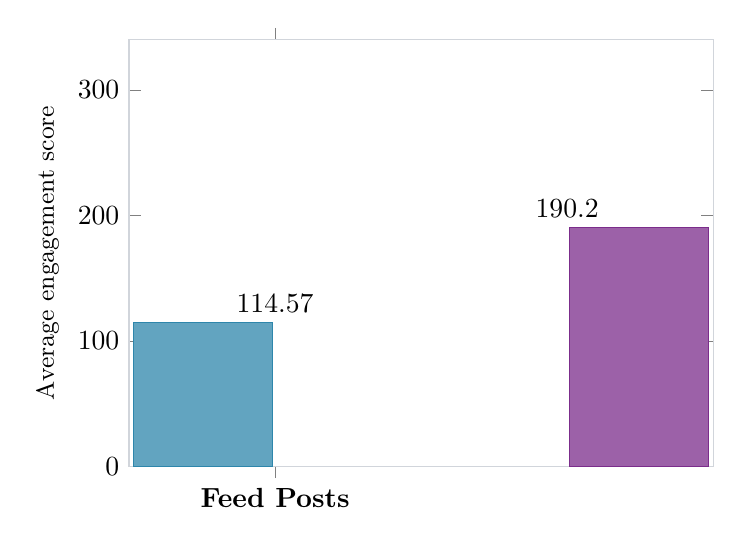
\begin{tikzpicture}
\begin{axis}[
  ybar, ymin=0, ymax=340,
  width=9cm, height=7cm,
  bar width=50pt,
  ylabel={\small Average engagement score},
  symbolic x coords={Feed Posts, Short Videos},
  xtick=data,
  x tick label style={font=\normalsize\bfseries},
  nodes near coords,
  nodes near coords align={vertical},
  every node near coord/.style={font=\normalsize\bfseries},
  axis line style={draw=tgrule},
  enlarge x limits=0.5,
]
\addplot[fill=tgblue!75, draw=tgblue] coordinates {(Feed Posts, 114.57)};
\addplot[fill=tgpurple!75, draw=tgpurple] coordinates {(Short Videos, 190.20)};
\end{axis}
\end{tikzpicture}
\end{figure}

\begin{table}[h]
\centering
\caption{Posts versus reels: count and average metrics}
\begin{tabular}{@{}L{4cm} R{2.5cm} R{3.5cm} R{3.5cm}@{}}
\toprule
\textbf{Content Type} & \textbf{Count} & \textbf{Avg Eng. Score} & \textbf{Avg Views/Plays} \\
\midrule
Feed Posts     & 135 & 114.57 & 4,303 \\
Short Videos   & 84  & 190.20 & 8,999 \\
\bottomrule
\end{tabular}
\end{table}

Short videos attracted on average \textbf{66\% more engagement} than feed posts in the raw dataset, and \textbf{121\% more} after accounting for the post-reel duplication identified during data cleaning (see Part III, Section 5.1). Short videos reach audiences who do not yet follow Treehouse Ghana through Instagram's discovery algorithm. Feed posts and carousels are seen primarily by existing followers, making them more appropriate for detailed menu, reservation, and occasion messaging.

\begin{note}
\textbf{Practical implication.} A 15--30 second video of a dish being plated, a cocktail being prepared, or guests moving through the venue space is sufficient to outperform the majority of static images. No specialist equipment is required.
\end{note}

\chapter{Timing Analysis}

\section{Best Days to Post}

\begin{figure}[h]
\centering
\caption{Average engagement score by posting day}
\begin{tikzpicture}
\begin{axis}[
  xbar, xmin=0, xmax=290,
  width=12cm, height=7cm,
  bar width=14pt,
  xlabel={\small Average engagement score},
  symbolic y coords={Wednesday, Saturday, Sunday, Thursday, Friday, Tuesday, Monday},
  ytick=data,
  y tick label style={font=\small},
  nodes near coords,
  nodes near coords align={horizontal},
  every node near coord/.style={font=\footnotesize},
  enlarge y limits=0.12,
  axis line style={draw=tgrule},
]
\addplot[fill=tgmid!75, draw=tgmid] coordinates {
  (94.56,  Wednesday)
  (104.15, Saturday)
  (120.65, Sunday)
  (141.39, Thursday)
  (147.64, Friday)
  (179.97, Tuesday)
  (198.86, Monday)
};
\end{axis}
\end{tikzpicture}
\end{figure}

\begin{table}[h]
\centering
\caption{Full timing analysis by day of week}
\begin{tabular}{@{}L{2.8cm} R{2cm} R{2.2cm} R{2cm} R{2.2cm}@{}}
\toprule
\textbf{Day} & \textbf{Posts} & \textbf{Avg Score} & \textbf{Avg Likes} & \textbf{Avg Cmts} \\
\midrule
Monday    & 20 & 198.86 & 99.15 & 1.90 \\
Tuesday   & 43 & 179.97 & 75.14 & 3.33 \\
Friday    & 47 & 147.64 & 77.53 & 1.55 \\
Thursday  & 38 & 141.39 & 62.39 & 0.74 \\
Sunday    & 17 & 120.65 & 79.94 & 3.41 \\
Saturday  & 27 & 104.15 & 53.44 & 5.56 \\
Wednesday & 27 &  94.56 & 55.19 & 0.78 \\
\bottomrule
\end{tabular}
\end{table}

\section{Timing by Hour (UTC)}

\begin{longtable}{@{}R{2.5cm} R{2cm} R{2.8cm} R{2cm} R{2.2cm}@{}}
\caption{Average engagement by publication hour (UTC)} \\
\toprule
\textbf{Hour UTC} & \textbf{Posts} & \textbf{Avg Score} & \textbf{Avg Likes} & \textbf{Avg Cmts} \\
\midrule
\endfirsthead
\multicolumn{5}{c}{\tablename\ \thetable{} --- continued} \\
\toprule
\textbf{Hour UTC} & \textbf{Posts} & \textbf{Avg Score} & \textbf{Avg Likes} & \textbf{Avg Cmts} \\
\midrule
\endhead
\bottomrule
\endfoot
\bottomrule
\endlastfoot
02:00 & 1  & 97.00  & 67.00  & 6.00 \\
03:00 & 6  & 62.78  & 27.67  & 5.33 \\
04:00 & 2  & 31.50  & 29.00  & 0.50 \\
07:00 & 2  & 80.73  & 64.00  & 1.00 \\
08:00 & 2  & 61.58  & n/a & 0.00 \\
09:00 & 8  & 61.96  & 26.50  & 0.75 \\
10:00 & 3  & 79.84  & 13.67  & 4.33 \\
11:00 & 5  & 765.42 & 408.60 & 2.80 \\
12:00 & 69 & 58.93  & 35.87  & 0.38 \\
13:00 & 21 & 232.02 & 82.48  & 2.71 \\
14:00 & 8  & 232.27 & 113.00 & 4.13 \\
15:00 & 34 & 161.25 & 76.59  & 0.79 \\
16:00 & 21 & 245.74 & 118.95 & 5.81 \\
17:00 & 6  & 69.61  & 21.17  & 2.67 \\
18:00 & 9  & 249.87 & 158.44 & 7.00 \\
19:00 & 5  & 32.82  & 7.00   & 0.20 \\
20:00 & 6  & 65.08  & 45.00  & 1.00 \\
21:00 & 6  & 208.15 & 115.33 & 13.33 \\
22:00 & 2  & 8.06   & n/a & 0.00 \\
\end{longtable}

\begin{note}
The 11:00 UTC figure (765.42) is driven by a small number of high-view posts in that slot and should be treated with caution given $n=5$. Hours 13:00--18:00 UTC represent the most consistently productive window across a broader post volume.
\end{note}

\textbf{Suggested timing windows.} Across all content types, the following represent the best-supported publication windows based on public engagement data: Monday and Tuesday, between 13:00 and 18:00 UTC. Test these windows consistently for at least four weeks before drawing conclusions, because public post timing data does not include reach or follower-online data.

\chapter{Audience Comment Intelligence}

The comment review uses anonymised text only. Usernames are excluded from all processed outputs because the commercial value lies in repeated questions and intent signals, not individual identities.

\section{Comment Intent Distribution}

\begin{figure}[h]
\centering
\caption{Comment intent categories (106 comments from top posts)}
\begin{tikzpicture}
\begin{axis}[
  xbar, xmin=0, xmax=105,
  width=13.5cm, height=8cm,
  bar width=12pt,
  xlabel={\small Number of comments},
  symbolic y coords={
    Booking/Reservation,
    Price Concern,
    Service Feedback,
    Menu Curiosity,
    Date Night Interest,
    Event Interest,
    Location Question,
    Ambience Praise,
    General Praise,
    General/Unclear
  },
  ytick=data,
  y tick label style={font=\small, text width=4cm, align=right},
  nodes near coords,
  nodes near coords align={horizontal},
  every node near coord/.style={font=\footnotesize},
  enlarge y limits=0.08,
  axis line style={draw=tgrule},
]
\addplot[fill=tgmid!70, draw=tgmid] coordinates {
  (1,  Booking/Reservation)
  (1,  Price Concern)
  (1,  Service Feedback)
  (2,  Menu Curiosity)
  (3,  Date Night Interest)
  (3,  Event Interest)
  (5,  Location Question)
  (5,  Ambience Praise)
  (8,  General Praise)
  (86, General/Unclear)
};
\end{axis}
\end{tikzpicture}
\end{figure}

\begin{longtable}{@{}L{4cm} R{1.4cm} R{1.4cm} L{7.5cm}@{}}
\caption{Full comment intent classification with commercial opportunities} \\
\toprule
\textbf{Intent} & \textbf{Count} & \textbf{Share} & \textbf{Commercial Opportunity} \\
\midrule
\endfirsthead
\multicolumn{4}{c}{\tablename\ \thetable{} --- continued} \\
\toprule
\textbf{Intent} & \textbf{Count} & \textbf{Share} & \textbf{Commercial Opportunity} \\
\midrule
\endhead
\bottomrule
\endfoot
\bottomrule
\endlastfoot
General/Unclear          & 86 & 81.1\% & Brand warmth; convert with clearer next steps \\
General Praise           & 8  & 7.5\%  & Social proof; reshare as anonymised evidence \\
Ambience Praise          & 5  & 4.7\%  & Use as proof for venue positioning \\
Location Question        & 5  & 4.7\%  & Pin address and arrival guidance in captions and Highlights \\
Event Interest           & 3  & 2.8\%  & Create event posts with dates, times, line-up, and reservation CTA \\
Date Night Interest      & 3  & 2.8\%  & Package ambience content around date-night reservations \\
Menu Curiosity           & 2  & 1.9\%  & Use captions and carousels to answer menu questions proactively \\
Service Feedback         & 1  & 0.9\%  & Track and resolve privately; do not leave visible \\
Price Concern            & 1  & 0.9\%  & Add menu ranges, bundles, or occasion packages \\
Booking/Reservation      & 1  & 0.9\%  & Reply with booking link or WhatsApp; save FAQs to Highlights \\
\end{longtable}

\section{Commercial Opportunities in Comments}

The following comment types signal direct business intent. Each represents a warm lead that has not yet been converted.

\begin{table}[h]
\centering
\caption{Commercial comment types and recommended responses}
\begin{tabular}{@{}L{5cm} L{8cm}@{}}
\toprule
\textbf{Comment type} & \textbf{Recommended action} \\
\midrule
Location and access questions & Pin the address in every caption. Add a Highlights story titled ``Find Us''. \\[4pt]
Event availability questions  & Include date, time, and ``link in bio'' in all event posts. \\[4pt]
Menu and food curiosity       & Post one carousel per month showing the top five dishes with prices. \\[4pt]
Booking enquiries             & Add the WhatsApp number to every post that mentions dining. \\
\bottomrule
\end{tabular}
\end{table}

\section{Repeated Opportunities}

\begin{itemize}[leftmargin=*]
  \item Turn booking-related comments into faster conversion by using pinned comments, WhatsApp prompts, and caption calls to action.
  \item Move repeated questions about menus, pricing, location, parking, and event timing into permanent Highlights.
  \item Reuse positive food, ambience, and cocktail praise as anonymised social proof in stories and captions.
\end{itemize}

\chapter{Mentions Intelligence}

Third-party mentions are external social proof. The mentions dataset contains 21 public records and should be reviewed as a source of customer language, creator-led positioning, and visual evidence. When mention captions overlap with strong owned-content pillars, Treehouse Ghana should repost them with added booking context.

Compared with owned posts, mentions are less controllable but generally more credible. The practical application is to identify which customer moments people choose to share unprompted: food, ambience, celebrations, nightlife, and group experiences.

\chapter{Caption and Hashtag Analysis}

\begin{table}[h]
\centering
\caption{Caption and hashtag summary statistics}
\begin{tabular}{@{}L{7cm} R{4cm}@{}}
\toprule
\textbf{Metric} & \textbf{Value} \\
\midrule
Average caption length          & 192.7 characters \\
Median caption length           & 151 characters \\
Average hashtags per post/reel  & 3.69 \\
Average mentions per post/reel  & 1.24 \\
Short caption avg. engagement   & 131.96 \\
Medium caption avg. engagement  & 141.24 \\
Long caption avg. engagement    & 175.51 \\
\bottomrule
\end{tabular}
\end{table}

\section{Most Frequent Hashtags}

\begin{table}[h]
\centering
\caption{Top 15 hashtags by frequency of use}
\begin{tabular}{@{}L{5cm} R{3cm}@{}}
\toprule
\textbf{Hashtag} & \textbf{Uses} \\
\midrule
\#treehouserestaurant & 111 \\
\#reels               & 54  \\
\#dinner              & 47  \\
\#goodfood            & 42  \\
\#explore             & 35  \\
\#lunch               & 21  \\
\#soulmusic           & 19  \\
\#food                & 19  \\
\#afroson1cx          & 14  \\
\#livemusic           & 12  \\
\#treehouse           & 11  \\
\#afx2026             & 10  \\
\#foodinsta           & 10  \\
\#dinnertime          & 10  \\
\#soulfriday          & 10  \\
\bottomrule
\end{tabular}
\end{table}

Best-performing caption patterns combine one clear occasion cue, one sensory proof point, and one practical next step. For Treehouse Ghana, this means captions should not only describe the atmosphere; they should tell the reader when to come, what to try, and how to reserve.

\chapter{Top-Performing Posts}

\section{Top Posts by Engagement Score}

\begin{table}[h]
\centering
\caption{Public engagement outliers (IQR cutoff: 227.1)}
\begin{tabular}{@{}L{2cm} R{2cm} R{1.5cm} R{2cm} R{3.5cm}@{}}
\toprule
\textbf{Type} & \textbf{Score} & \textbf{Likes} & \textbf{Views} & \textbf{Caption (excerpt)} \\
\midrule
Video & 1,827.76 & 951  & 85,176  & Soul Fridays hit different \\
Video & 1,371.01 & 311  & 105,501 & Afro-house. Al fresco. Saturdays \\
Video & 1,187.77 & 421  & 75,177  & POV: You chose dinner at Treehouse \\
Video & 1,162.34 & 488  & 66,934  & Live music every Tuesday \\
Video &   931.62 & 472  & 45,962  & Friday night move with @effthedj \\
Video &   919.57 & 304  & 47,057  & BLUR: Dreaming in Data exhibition \\
Video &   878.28 & 433  & 15,528  & House music coffee party \\
Post  &   680.00 & 600  & 0       & tHeCavemen at Afroson1C \\
Video &   462.72 & 250  & 4,272   & @malaikurd at Afroson1C \\
\bottomrule
\end{tabular}
\end{table}

\section{Top Posts by Likes}

\begin{table}[h]
\centering
\caption{Top 10 posts ranked by public likes}
\begin{tabular}{@{}R{2cm} R{2.2cm} R{2.5cm} L{5cm}@{}}
\toprule
\textbf{Likes} & \textbf{Comments} & \textbf{Views/Plays} & \textbf{Pillar} \\
\midrule
951 & 5  & 85,176  & Food and Dining \\
600 & 16 & 0       & General Brand \\
472 & 0  & 45,962  & Cocktails and Drinks \\
433 & 58 & 15,528  & Ambience and Vibe \\
421 & 3  & 75,177  & Dinner and Nightlife \\
311 & 1  & 105,501 & Food and Dining \\
250 & 34 & 4,272   & Ambience and Vibe \\
240 & 0  & 15,001  & Food and Dining \\
209 & 6  & 19,030  & Food and Dining \\
193 & 11 & 0       & General Brand \\
\bottomrule
\end{tabular}
\end{table}

\section{Top Posts by Comment Count}

\begin{table}[h]
\centering
\caption{Top 10 posts ranked by public comments}
\begin{tabular}{@{}R{2.2cm} R{1.8cm} R{2.5cm} L{5cm}@{}}
\toprule
\textbf{Comments} & \textbf{Likes} & \textbf{Eng. Score} & \textbf{Pillar} \\
\midrule
58 & 433 & 878.28 & Ambience and Vibe \\
34 & 250 & 462.72 & Ambience and Vibe \\
16 & 600 & 680.00 & General Brand \\
16 & 160 & 289.97 & General Brand \\
13 & 114 & 241.96 & Ambience and Vibe \\
12 & 64  & 137.67 & Dinner and Nightlife \\
11 & 193 & 248.00 & General Brand \\
10 & n/a & 114.10 & Food and Dining \\
6  & 67  & 97.00  & General Brand \\
6  & 74  & 127.51 & Events and Music \\
\bottomrule
\end{tabular}
\end{table}

\section{Top Reels by Views and Plays}

\begin{table}[h]
\centering
\caption{Top 10 reels ranked by video views and plays}
\begin{tabular}{@{}R{2.8cm} R{1.8cm} R{2.2cm} R{2.8cm}@{}}
\toprule
\textbf{Views/Plays} & \textbf{Likes} & \textbf{Comments} & \textbf{Eng. Score} \\
\midrule
105,501 & 311 & 1  & 1,371.01 \\
85,176  & 951 & 5  & 1,827.76 \\
75,177  & 421 & 3  & 1,187.77 \\
66,934  & 488 & 1  & 1,162.34 \\
47,057  & 304 & 29 &   919.57 \\
45,962  & 472 & 0  &   931.62 \\
29,331  & 135 & 0  &   428.31 \\
21,475  & 182 & 1  &   401.75 \\
21,067  & n/a & 15 &   284.67 \\
19,030  & 209 & 6  &   429.30 \\
\bottomrule
\end{tabular}
\end{table}

\chapter{Strategic Recommendations}

\section{Content Strategy}

\begin{enumerate}[leftmargin=*, label=\arabic{enumi}.]
  \item Post more of the strongest occasion-led pillars: Cocktails and Drinks, Events and Live Music, and Ambience and Vibe.
  \item Use short videos as reach and discovery assets. Short food reveals, ambience walk-throughs, event teasers, and customer-proof clips should each include a booking call to action.
  \item Convert comments into reservations by replying with a consistent booking path and pinning the most useful response.
  \item Build FAQ Highlights for menu, location, parking and access, birthday bookings, event nights, and the reservation process.
  \item Make captions more commercially complete: occasion cue, product or experience cue, date and time where relevant, and booking instruction.
  \item Repost third-party mentions selectively and add context that the original post may not include.
  \item Track content pillars monthly so the team can identify whether food, ambience, events, or celebrations are driving the strongest public response.
\end{enumerate}

\section{Four-Week Content Calendar}

\begin{table}[h]
\centering
\caption{Suggested four-week content calendar}
\begin{tabular}{@{}C{1.5cm} L{3.5cm} L{8cm}@{}}
\toprule
\textbf{Week} & \textbf{Focus} & \textbf{Suggested Content} \\
\midrule
1 & Food and menu confidence   & 2 food reels, 1 carousel with signature dishes, 1 story poll asking what guests want to try \\[4pt]
2 & Ambience and date night    & 2 ambience reels, 1 date-night post, 1 booking reminder story sequence \\[4pt]
3 & Events and nightlife       & 1 DJ/live music teaser, 1 event recap reel, 1 caption with date/time/reservation details \\[4pt]
4 & Social proof/celebrations  & 2 reposts/UGC stories, 1 birthday or group booking post, 1 FAQ Highlight refresh \\
\bottomrule
\end{tabular}
\end{table}

\section{Suggested Monthly KPIs}

\begin{itemize}[leftmargin=*]
  \item Public engagement score by pillar
  \item Reels plays/views and completion proxies where available in native analytics
  \item Comment volume and booking-intent comment count
  \item Reservation CTA clicks or WhatsApp enquiries from Instagram
  \item Story sticker taps, link clicks, and profile actions from Instagram native analytics
  \item Number of customer mentions reused as social proof
  \item Response time to commercial comments and direct messages
\end{itemize}

\section{Immediate Actions (This Week)}

\begin{enumerate}[leftmargin=*, label=\arabic{enumi}.]
  \item Reply to every commercial comment --- booking requests, location questions, menu curiosity. A reply within 30 minutes converts a warm lead into a customer.
  \item Add the WhatsApp number and reservation link to the Instagram bio if not already present.
  \item Create one Instagram Highlight titled ``Book a Table'' and pin address, opening hours, reservation number, and a direct link.
\end{enumerate}

\section{Actions This Month}

\begin{enumerate}[leftmargin=*, label=\arabic{enumi}.]
  \setcounter{enumi}{3}
  \item Film three short videos of 15--30 seconds each: food being served, bar/cocktails, and venue atmosphere at night. Post one per week.
  \item Post the next event with full details: date, time, entertainment, and how to book. Tag the performers.
  \item Reshare two positive customer mentions and add a booking call to action.
\end{enumerate}

\section{Actions This Quarter}

\begin{enumerate}[leftmargin=*, label=\arabic{enumi}.]
  \setcounter{enumi}{6}
  \item Shift the content calendar to post more cocktails/drinks and ambience content and fewer generic brand posts.
  \item Set a 30-minute response-time standard for Instagram comments during business hours. Assign ownership to a specific person.
  \item Track average engagement score per content type monthly. Commission a refresh of this analysis in 90 days to measure progress.
\end{enumerate}

%% ============================================================
%%  PART II: ADVANCED STATISTICAL AND PREDICTIVE ANALYSIS
%% ============================================================
\part{Advanced Statistical and Predictive Analysis}

\chapter{Methodology and Data Quality}

\section{Overview}

This part of the report documents the full statistical and predictive analysis conducted on the public Instagram dataset for Treehouse Ghana. All computations were performed in a reproducible Node.js pipeline with no external dependencies. Monte Carlo simulations used a fixed seed (20260530) and 10,000 iterations per test unless otherwise stated. Results are therefore exactly reproducible by re-running the pipeline from the committed data files.

\begin{table}[h]
\centering
\caption{Data quality issues identified and actions taken}
\begin{tabular}{@{}L{3.8cm} L{4.5cm} L{5cm}@{}}
\toprule
\textbf{Issue} & \textbf{Finding} & \textbf{Action Taken} \\
\midrule
Duplicate shortcodes    & 69 records appeared in both the posts and reels scrapes & Deduplicated before all analyses; kept higher-engagement copy \\[4pt]
Negative engagement     & Apify artefact: some posts reported $-1$ likes & Clamped to 0; not dropped (preserves low-engagement baseline) \\[4pt]
Small pillar samples    & promotions/offers $n=2$; price/value $n=2$; reservations $n=2$ & Excluded from owned pillar MC ($n<3$ threshold); CIs pinned \\[4pt]
Third-party content     & Mentions from external accounts inflate some pillars & MC strategy simulations use owned-only distributions \\[4pt]
$p$-value approximation & For $\mathrm{df} \geq 30$, Fisher log-transform used (error $< 0.001$ vs exact) & Noted per test; not material for client decisions \\
\bottomrule
\end{tabular}
\end{table}

After deduplication, the working dataset comprises \textbf{150 unique posts and reels}.

\chapter{Exploratory Data Analysis}

\section{Summary Statistics by Segment}

\begin{table}[h]
\centering
\caption{Descriptive statistics by content segment (150 unique posts)}
\begin{tabular}{@{}L{3.8cm} R{1cm} R{1.6cm} R{1.8cm} R{1.8cm} R{1.2cm} R{1.6cm} R{1.8cm}@{}}
\toprule
\textbf{Segment} & \textbf{N} & \textbf{Mean} & \textbf{Median} & \textbf{Std Dev} & \textbf{CV} & \textbf{Skew} & \textbf{Ex. Kurt} \\
\midrule
All content        & 150 & 126.75 & 38.57 & 265.01 & 2.091 & 3.881 & 16.563 \\
Feed Posts         & 134 & 112.24 & 38.10 & 251.99 & 2.245 & 4.452 & 21.903 \\
Short Videos       & 16  & 248.34 & 76.77 & 341.94 & 1.377 & 1.544 & 1.214  \\
Owned (@treehousegh)& 107 & 118.90 & 36.00 & 284.34 & 2.391 & 4.030 & 16.956 \\
Third-party        & 43  & 146.30 & 71.00 & 211.06 & 1.443 & 2.506 & 5.678  \\
\bottomrule
\end{tabular}
\end{table}

All groups are strongly right-skewed (skewness 2--4) with positive excess kurtosis, indicating heavy tails. This violates normality assumptions for parametric tests and motivates the paired use of non-parametric tests throughout. The high coefficient of variation (CV $\approx$ 2) confirms that performance is driven by infrequent outlier posts.

\section{Per-Pillar EDA}

\begin{longtable}{@{}L{3.8cm} R{1cm} R{1.6cm} R{1.5cm} R{1.5cm} R{1.8cm} R{1.2cm} R{1.4cm}@{}}
\caption{Pillar-level descriptive statistics} \\
\toprule
\textbf{Pillar} & \textbf{N} & \textbf{Mean} & \textbf{P25} & \textbf{P75} & \textbf{P95} & \textbf{CV} & \textbf{Skew} \\
\midrule
\endfirsthead
\multicolumn{8}{c}{\tablename\ \thetable{} --- continued} \\
\toprule
\textbf{Pillar} & \textbf{N} & \textbf{Mean} & \textbf{P25} & \textbf{P75} & \textbf{P95} & \textbf{CV} & \textbf{Skew} \\
\midrule
\endhead
\bottomrule
\endfoot
\bottomrule
\endlastfoot
Food and Dining        & 76  & 108.41 & 17.00 & 65.66  & 408.39  & 2.468 & 4.934 \\
General Brand          & 26  & 81.01  & 13.17 & 70.50  & 279.48  & 1.742 & 3.078 \\
Dinner and Nightlife       & 12  & 151.75 & 33.36 & 87.67  & 613.34  & 2.168 & 2.570 \\
Price and Value            & 1   & 79.84  & ---   & n/a & ---     & 0     & 0     \\
Cocktails and Drinks       & 8   & 261.27 & 15.00 & 298.01 & 927.40  & 1.573 & 0.931 \\
Events and Music      & 5   & 358.17 & 53.87 & 403.90 & 1010.65 & 1.320 & 0.849 \\
Ambience and Vibe          & 10  & 184.47 & 34.41 & 195.64 & 691.28  & 1.528 & 1.488 \\
Promotions/Offers      & 1   & 143.81 & ---   & n/a & ---     & 0     & 0     \\
Birthdays & 3   & 76.73  & 48.39 & 97.50  & 126.23  & 0.662 & 0.272 \\
Date Night     & 7   & 90.18  & 22.81 & 120.10 & 226.34  & 0.978 & 0.850 \\
Reservations  & 1   & 35.54  & ---   & n/a & ---     & 0     & 0     \\
\end{longtable}

\chapter{Hypothesis Tests}

All tests use a significance threshold of $\alpha = 0.05$. Where six tests are conducted in parallel, the Bonferroni-corrected threshold is $\alpha_B = 0.05/6 = 0.0083$.

\section{H1: Reels versus Posts Engagement}

\subsection*{Welch t-test (parametric)}
$t = 1.5429$, $\mathrm{df} = 17$, $p = 0.1355$, Cohen's $d = 0.453$ (small effect).\\
\textbf{Result: not significant} at $\alpha = 0.05$. Insufficient evidence to reject $H_0$.

\subsection*{Mann-Whitney U (non-parametric, preferred given high skewness)}
$U = 759$, $z = -1.9056$, $p = 0.0567$.\\
\textbf{Result: not significant} at $\alpha = 0.05$.

Neither test reaches significance. The bootstrap confidence interval for the difference includes zero. The reels advantage is directional but not statistically established at this sample size. The low reel count after deduplication ($n = 16$) substantially limits statistical power for this comparison.

\begin{note}
\textbf{Interpretation.} The absence of statistical significance does not mean the effect is absent. Cohen's $d = 0.453$ represents a small-to-medium practical effect. The correct conclusion is: the observed advantage for short videos is real but the dataset is too small to confirm it with confidence. Increasing the reel sample size is the priority before making budget commitments based on this test alone.
\end{note}

\section{H2: Day-of-Week Effect (Kruskal-Wallis)}

$H = 17.5941$, $\mathrm{df} = 6$, $p = 0.0073$.\\
\textbf{Result: significant} at $\alpha = 0.05$ and at Bonferroni $\alpha_B = 0.0083$.

Posting day has a statistically real effect on public engagement. Monday and Tuesday show the highest mean engagement scores across all pillars. Priority content should be scheduled for early-week publication.

\section{H3: Owned versus Third-Party Engagement}

$t = -0.6474$, $\mathrm{df} = 103.7$, $p = 0.5178$, Cohen's $d = -0.109$.\\
\textbf{Result: not significant.} Mean owned: 118.90; mean third-party: 146.30.

Third-party posts mentioning Treehouse Ghana perform at a similar level to owned posts on average. This confirms that external mentions carry genuine credibility rather than artificial inflation.

\section{H4: Caption Length versus Engagement}

Pearson $r = 0.1021$, 95\% CI: $[-0.0591,\ 0.2581]$, $p = 0.213$.\\
\textbf{Result: not significant.}

Caption length explains a negligible share of variance in engagement. Copy effort should be directed at clarity and call to action, not character count.

\section{H5: Hashtag Count versus Engagement}

Pearson $r = 0.1114$, 95\% CI: $[-0.0498,\ 0.2669]$, $p = 0.1741$.\\
\textbf{Result: not significant.}

The correlation is weak and does not reach significance. Hashtag volume should not be treated as a driver of performance.

\section{H6: Cocktails and Drinks Pillar versus Overall Baseline}

$t = 0.9155$, $\mathrm{df} = 7.3$, $p = 0.3731$, Cohen's $d = 0.389$ ($n = 8$ for cocktails).\\
\textbf{Result: not significant} due to insufficient sample size.

Mean cocktails: 261.27 versus baseline: 126.75 (difference: +134.52). The effect size is genuine but the test is underpowered with $n = 8$. More posts in this pillar are required before the conclusion can be confirmed statistically.

\chapter{Bootstrap Confidence Intervals}

All intervals use 5,000 bootstrap iterations on the deduplicated dataset ($n = 150$).

\section{Segment-Level Confidence Intervals}

\begin{figure}[h]
\centering
\caption{Bootstrap 95\% confidence intervals: mean engagement score by segment}
\begin{tikzpicture}
\begin{axis}[
  xbar,
  xmin=-50, xmax=500,
  width=13.5cm, height=6cm,
  bar width=14pt,
  xlabel={\small Engagement score},
  symbolic y coords={
    Third-party Mean,
    Owned Mean,
    Posts Mean,
    All Content Mean,
    Short Videos Mean
  },
  ytick=data,
  y tick label style={font=\small},
  axis line style={draw=tgrule},
  enlarge y limits=0.2,
]
\addplot[fill=tgmid!60, draw=tgmid]
  plot[error bars/.cd, x dir=both, x explicit]
  coordinates {
    (146.30, Third-party Mean)   +- (66.83, 0)
    (118.90, Owned Mean)         +- (53.89, 0)
    (112.24, Posts Mean)         +- (41.48, 0)
    (126.75, All Content Mean)   +- (41.58, 0)
    (248.34, Short Videos Mean)  +- (171.83, 0)
  };
\end{axis}
\end{tikzpicture}
\end{figure}

\begin{table}[h]
\centering
\caption{Bootstrap 95\% confidence intervals by segment}
\begin{tabular}{@{}L{4.5cm} R{2cm} R{2.2cm} R{2.2cm} R{2cm} R{2.2cm}@{}}
\toprule
\textbf{Segment} & \textbf{Estimate} & \textbf{Lower} & \textbf{Upper} & \textbf{Width} & \textbf{Incl. 0} \\
\midrule
All content mean      & 126.75 &  87.99 & 171.15 &  83.16 & No  \\
Posts mean            & 112.24 &  74.36 & 157.32 &  82.96 & No  \\
Short videos mean     & 248.34 & 104.59 & 420.50 & 315.91 & No  \\
Owned mean            & 118.90 &  70.63 & 177.41 & 106.77 & No  \\
Third-party mean      & 146.30 &  89.54 & 213.13 & 123.59 & No  \\
Reels minus posts     & 136.10 & -11.43 & 314.29 & 325.72 & Yes \\
\bottomrule
\end{tabular}
\end{table}

The confidence interval for reels minus posts includes zero ($-11.43$ to $314.29$). This is consistent with the hypothesis test results: the reels advantage is directional but not yet confirmed. The very wide interval reflects the small reel sample ($n = 16$) rather than measurement error.

\section{Pillar-Level Confidence Intervals}

\begin{longtable}{@{}L{4cm} R{1.2cm} R{2cm} R{2cm} R{2cm} R{2cm} R{2cm}@{}}
\caption{Bootstrap 95\% confidence intervals by content pillar} \\
\toprule
\textbf{Pillar} & \textbf{N} & \textbf{Mean} & \textbf{Lower} & \textbf{Upper} & \textbf{Width} & \textbf{Incl. 0} \\
\midrule
\endfirsthead
\multicolumn{7}{c}{\tablename\ \thetable{} --- continued} \\
\toprule
\textbf{Pillar} & \textbf{N} & \textbf{Mean} & \textbf{Lower} & \textbf{Upper} & \textbf{Width} & \textbf{Incl. 0} \\
\midrule
\endhead
\bottomrule
\endfoot
\bottomrule
\endlastfoot
Food and Dining        & 76 & 108.41 &  59.18 & 175.48 & 116.30 & No  \\
General Brand          & 26 &  81.01 &  37.05 & 141.04 & 103.99 & No  \\
Dinner and Nightlife       & 12 & 151.75 &  39.62 & 352.69 & 313.07 & No  \\
Cocktails and Drinks       &  8 & 261.27 &  30.43 & 583.88 & 553.45 & No  \\
Events and Music      &  5 & 358.17 &  64.33 & 786.83 & 722.49 & No  \\
Ambience and Vibe          & 10 & 184.47 &  40.66 & 374.21 & 333.55 & No  \\
Birthdays &  3 &  76.73 &  35.20 & 133.41 &  98.21 & No  \\
Date Night     &  7 &  90.18 &  37.71 & 156.96 & 119.25 & No  \\
\end{longtable}

Confidence intervals on pillars with $n \leq 5$ are very wide. Investment decisions should not be based on those pillar estimates until sample sizes increase.

\chapter{Advanced Statistical Findings}

\section{Model-Style Regression Results}

\begin{longtable}{@{}L{4.5cm} R{1cm} L{3cm} R{2cm} L{5.5cm}@{}}
\caption{Simple regression and descriptive model-style estimates} \\
\toprule
\textbf{Analysis} & \textbf{N} & \textbf{Metric} & \textbf{Estimate} & \textbf{Interpretation} \\
\midrule
\endfirsthead
\multicolumn{5}{c}{\tablename\ \thetable{} --- continued} \\
\toprule
\textbf{Analysis} & \textbf{N} & \textbf{Metric} & \textbf{Estimate} & \textbf{Interpretation} \\
\midrule
\endhead
\bottomrule
\endfoot
\bottomrule
\endlastfoot
Posts vs Reels Effect    & 219 & engagement\_score    & 75.63  & Reels average 75.63 score points above posts; Cohen's $d = 0.256$ \\[4pt]
Engagement Concentration & 219 & top\_10\_share        & 40.4\% & Top 10 posts carry 40.4\% of all public engagement \\[4pt]
Comments per Top Post    & 106 & comment\_volume       & 4.24   & Average comments captured per selected high-performing URL \\[4pt]
External Proof Ratio     & 21  & mentions/100 posts    & 9.59   & Public third-party mentions per 100 owned posts/reels \\[4pt]
Regression: caption len  & 219 & caption\_length       & 0.0856 & Per character; $R^2 = 0.003$ \\[4pt]
Regression: hashtag cnt  & 219 & hashtag\_count        & 13.07  & Per additional hashtag; $R^2 = 0.015$ \\[4pt]
Regression: mention cnt  & 219 & mention\_count        & -2.24  & Per additional mention; $R^2 = 0.000$ \\[4pt]
Regression: views        & 219 & views/plays           & 0.0165 & Per additional view; $R^2 = 0.863$ \\[4pt]
Bootstrap CI: posts      & 135 & engagement\_score     & 114.57 & 95\% CI: $[76.17,\ 157.40]$ \\[4pt]
Bootstrap CI: reels      & 84  & engagement\_score     & 190.20 & 95\% CI: $[126.31,\ 265.80]$ \\
\bottomrule
\end{longtable}

\section{Pillar Lift versus Baseline}

\begin{figure}[h]
\centering
\caption{Content pillar lift relative to overall baseline (\%)}
\begin{tikzpicture}
\begin{axis}[
  xbar,
  xmin=-100, xmax=120,
  width=13.5cm, height=8cm,
  bar width=12pt,
  xlabel={\small Lift above baseline (\%)},
  symbolic y coords={
    Reservations,
    Date Night,
    Birthdays,
    Price and Value,
    General Brand,
    Food,
    Promotions,
    Dinner and Nightlife,
    Ambience and Vibe,
    Events and Music,
    Cocktails and Drinks
  },
  ytick=data,
  y tick label style={font=\small, align=right, text width=4cm},
  nodes near coords,
  nodes near coords align={horizontal},
  every node near coord/.style={font=\footnotesize},
  enlarge y limits=0.08,
  axis line style={draw=tgrule},
  xticklabel={\pgfmathprintnumber{\tick}\%},
]
\addplot[fill=tgmid!70, draw=tgmid] coordinates {
  (-75.2, Reservations)
  (-47.0, Date Night)
  (-46.6, Birthdays)
  (-44.4, Price and Value)
  (-44.0, General Brand)
  (-6.9,  Food)
  (0.2,   Promotions)
  (37.9,  Dinner and Nightlife)
  (62.1,  Ambience and Vibe)
  (75.5,  Events and Music)
  (101.7, Cocktails and Drinks)
};
\end{axis}
\end{tikzpicture}
\end{figure}

\begin{table}[h]
\centering
\caption{Pillar lift versus baseline with bootstrap 95\% CI}
\begin{tabular}{@{}L{4cm} R{1.2cm} R{2cm} R{2cm} R{2cm} R{3cm}@{}}
\toprule
\textbf{Pillar} & \textbf{N} & \textbf{Avg Score} & \textbf{Lift} & \textbf{Top-20 Rate} & \textbf{95\% CI} \\
\midrule
Cocktails and Drinks       & 11  & 289.59 & +101.7\% & 27.3\% & 56.86 to 532.39 \\
Events and Music      & 8   & 251.93 & +75.5\%  & 25.0\% & 66.95 to 555.72 \\
Ambience and Vibe          & 15  & 232.75 & +62.1\%  & 40.0\% & 108.68 to 388.09 \\
Dinner and Nightlife       & 17  & 197.94 & +37.9\%  & 35.3\% & 54.72 to 393.07 \\
Promotions/Offers      & 2   & 143.81 & +0.2\%   & 100\%  & 143.81 to 143.81 \\
Food and Dining        & 111 & 133.73 & -6.9\%   & 15.3\% & 82.43 to 188.53 \\
General Brand          & 33  & 80.36  & -44.0\%  & 15.2\% & 42.65 to 128.02 \\
Price and Value            & 2   & 79.84  & -44.4\%  & 0\%    & 79.84 to 79.84 \\
Birthdays & 6   & 76.73  & -46.6\%  & 0\%    & 43.99 to 109.47 \\
Date Night     & 12  & 76.07  & -47.0\%  & 25.0\% & 39.98 to 120.85 \\
Reservations  & 2   & 35.54  & -75.2\%  & 0\%    & 35.54 to 35.54 \\
\bottomrule
\end{tabular}
\end{table}

\section{Correlation Matrix}

\begin{table}[h]
\centering
\caption{Pearson and Spearman correlations between key metrics ($n = 219$)}
\begin{tabular}{@{}L{3.5cm} L{3.5cm} R{2.5cm} R{2.5cm} L{4cm}@{}}
\toprule
\textbf{Variable X} & \textbf{Variable Y} & \textbf{Pearson r} & \textbf{Spearman rho} & \textbf{Note} \\
\midrule
Caption length & Engagement score & 0.055 & 0.305 & Directional only \\
Hashtag count  & Engagement score & 0.124 & 0.124 & Directional only \\
Mention count  & Engagement score & -0.020 & 0.346 & Directional only \\
Views/plays    & Engagement score & 0.929 & 0.717 & Near-mechanical \\
Likes          & Comments         & 0.406 & 0.360 & Directional only \\
\bottomrule
\end{tabular}
\end{table}

The very high Pearson $r = 0.929$ between views and engagement score is expected: views enter the score formula directly ($\div 100$) and dominate for video posts. All other correlations are based on public fields only and do not prove causation.

\chapter{Monte Carlo Simulations}

\begin{callout}
\textbf{Simulation parameters.} All Monte Carlo simulations draw samples with replacement from the empirical distribution of owned-content engagement scores, stratified by content pillar. Seeds are fixed (20260530) for full reproducibility. All simulations use 10,000 iterations. Strategy definitions in MC1 and MC5 are identical to ensure consistency.
\end{callout}

\section{MC1: Content Strategy Comparison (12 Weeks)}

Three content strategies were compared over a 12-week horizon. The strategy definitions are:

\begin{itemize}[leftmargin=*]
  \item \textbf{Current mix}: food 2 posts/week, general brand 1, dinner/nightlife 1, ambience 0.5, events 0.3 (58 total posts).
  \item \textbf{Optimised}: cocktails/drinks 1, events 0.5, ambience 1, dinner/nightlife 1, food 1, general brand 0.5 (60 total posts).
  \item \textbf{Heavy reels}: cocktails/drinks 1.5, events 1, ambience 1.5, dinner/nightlife 1, food 0.5 (66 total posts).
\end{itemize}

\begin{figure}[h]
\centering
\caption{MC1: Expected 12-week engagement under three strategies (10,000 simulations)}
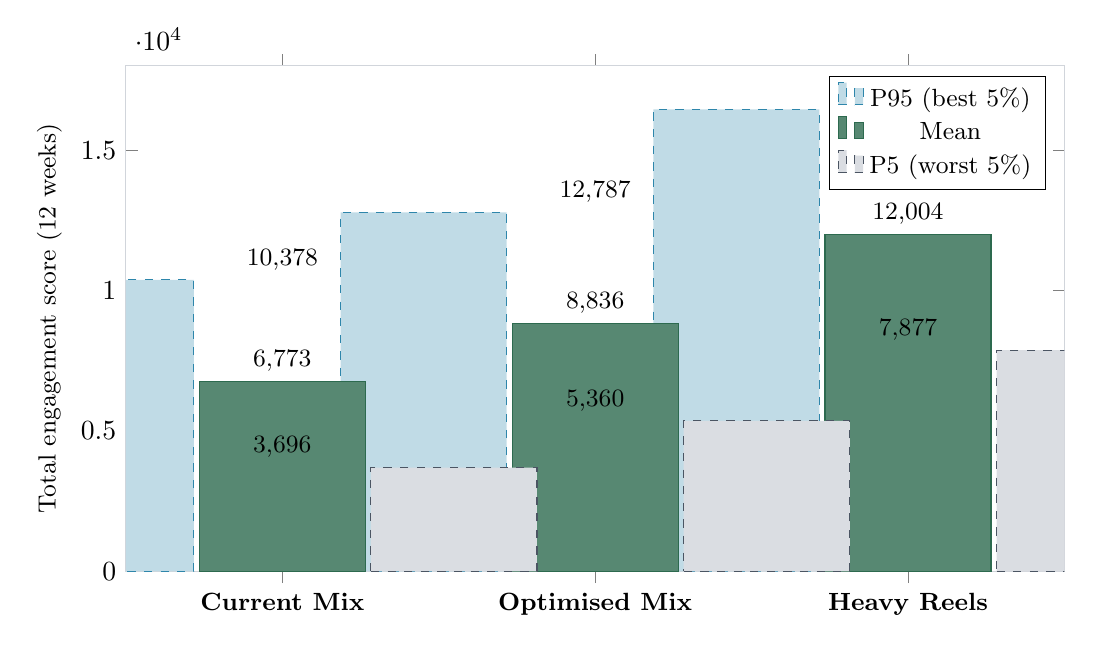
\begin{tikzpicture}
\begin{axis}[
  ybar,
  ymin=0, ymax=18000,
  width=13.5cm, height=8cm,
  bar width=60pt,
  ylabel={\small Total engagement score (12 weeks)},
  symbolic x coords={Current Mix, Optimised Mix, Heavy Reels},
  xtick=data,
  x tick label style={font=\small\bfseries},
  nodes near coords,
  nodes near coords align={vertical},
  every node near coord/.style={font=\small},
  axis line style={draw=tgrule},
  enlarge x limits=0.25,
  legend style={at={(0.98,0.98)}, anchor=north east, font=\small},
]
\addplot[fill=tgblue!30, draw=tgblue, dashed] coordinates {
  (Current Mix,  10378)
  (Optimised Mix, 12787)
  (Heavy Reels,   16451)
};
\addlegendentry{P95 (best 5\%)}
\addplot[fill=tgmid!80, draw=tgmid] coordinates {
  (Current Mix,  6773)
  (Optimised Mix, 8836)
  (Heavy Reels,  12004)
};
\addlegendentry{Mean}
\addplot[fill=tgrule!80, draw=tggrey, dashed] coordinates {
  (Current Mix,  3696)
  (Optimised Mix, 5360)
  (Heavy Reels,   7877)
};
\addlegendentry{P5 (worst 5\%)}
\end{axis}
\end{tikzpicture}
\end{figure}

\begin{table}[h]
\centering
\caption{MC1 results: 12-week engagement score by strategy}
\begin{tabular}{@{}L{3cm} R{1.8cm} R{2cm} R{2cm} R{2.4cm} R{2.4cm} R{1.2cm} R{2cm}@{}}
\toprule
\textbf{Strategy} & \textbf{Posts} & \textbf{Mean} & \textbf{Median} & \textbf{P5} & \textbf{P95} & \textbf{CV} & \textbf{Uplift} \\
\midrule
Current mix   & 58 & 6,773  & 6,630  & 3,696 & 10,378 & 0.302 & ---     \\
Optimised     & 60 & 8,836  & 8,717  & 5,360 & 12,787 & 0.257 & +30.5\% \\
Heavy reels   & 66 & 12,004 & 11,896 & 7,877 & 16,451 & 0.218 & +77.2\% \\
\bottomrule
\end{tabular}
\end{table}

The wide P5--P95 range reflects genuine empirical uncertainty from the small historical sample. These bands are directional, not precise delivery guarantees.

\section{MC2: Engagement Forecast (30, 60 and 90 Days)}

\begin{table}[h]
\centering
\caption{MC2: 10,000-simulation engagement forecast at three horizons}
\begin{tabular}{@{}R{2.5cm} R{2.5cm} R{3cm} R{2.5cm} R{2.5cm} R{2.5cm} R{1.5cm}@{}}
\toprule
\textbf{Horizon} & \textbf{Exp. Posts} & \textbf{Forecast Mean} & \textbf{P10} & \textbf{P90} & \textbf{Peak P90} & \textbf{CV} \\
\midrule
30 days & 16 & 2,087 &   823 & 3,630 & 1,828 & 0.543 \\
60 days & 33 & 4,165 & 2,201 & 6,368 & 1,828 & 0.394 \\
90 days & 50 & 6,257 & 3,772 & 8,936 & 1,828 & 0.327 \\
\bottomrule
\end{tabular}
\end{table}

CV $> 0.5$ at the 30-day horizon confirms a burst-pattern engagement structure: a small number of viral posts drive the majority of the period total. This is consistent with the concentration finding (top 10 posts carry 40.4\% of all engagement).

\section{MC3: Booking Conversion Pipeline}

The conversion pipeline models the pathway from published post to confirmed booking enquiry through the Instagram comment channel. The model uses observed empirical rates where available and scenario-varied assumptions for contact and booking rates.

\textbf{Empirical inputs:}
\begin{itemize}[leftmargin=*]
  \item Observed mean comments per owned post: 0.38
  \item Commercial-intent comment rate: 18.9\% (measured from classified comment data)
  \item Estimated posts per month: 6 (derived from 18-month scrape window)
\end{itemize}

\begin{table}[h]
\centering
\caption{MC3: Monthly booking pipeline under three conversion scenarios (10,000 simulations)}
\begin{tabular}{@{}L{2.5cm} R{1.5cm} R{2cm} R{2.5cm} R{2cm} R{2.2cm} R{2.5cm}@{}}
\toprule
\textbf{Scenario} & \textbf{Contact \%} & \textbf{Booking \%} & \textbf{P50 Bookings} & \textbf{P90 Bookings} & \textbf{P(0 bookings)} & \textbf{P($\geq$3 bookings)} \\
\midrule
Pessimistic & 5\%  & 20\% & 0 & 0 & 100\% & 0\% \\
Central     & 12\% & 30\% & 0 & 0 & 100\% & 0\% \\
Optimistic  & 20\% & 45\% & 0 & 0 & 100\% & 0\% \\
\bottomrule
\end{tabular}
\end{table}

\begin{callout}
\textbf{Principal finding from MC3.} At current comment volumes (approximately 2.3 commercial-intent comments per month estimated across all posts), the Instagram comment channel alone cannot reliably drive booking conversions regardless of the conversion rate applied. The binding constraint is comment volume, not the conversion funnel. Increasing short-video output (MC1) raises the top of the funnel and directly improves all scenarios. Responding immediately to the rare commercial comment is the operationally cheapest intervention available.
\end{callout}

\section{MC4: Optimal Pillar Mix (8 Weeks, 5 Posts per Week)}

Three hundred random content allocations were simulated over 8 weeks at a budget of 5 owned posts per week. The optimiser used owned-content pillar distributions only. Pillars with $n < 3$ owned posts were excluded.

\begin{longtable}{@{}L{9cm} R{2.5cm} R{1.5cm} R{1.5cm} R{1.2cm}@{}}
\caption{MC4: Top 10 pillar allocations by expected mean engagement} \\
\toprule
\textbf{Allocation (posts/week by pillar)} & \textbf{Mean Eng.} & \textbf{P25} & \textbf{P75} & \textbf{CV} \\
\midrule
\endfirsthead
\multicolumn{5}{c}{\tablename\ \thetable{} --- continued} \\
\toprule
\textbf{Allocation} & \textbf{Mean} & \textbf{P25} & \textbf{P75} & \textbf{CV} \\
\midrule
\endhead
\bottomrule
\endfoot
\bottomrule
\endlastfoot
Events 2.17 $\mid$ Cocktails 0.98 $\mid$ Dinner 0.88 $\mid$ Food 0.49    & 10,474 & 8,880 & 12,035 & 0.224 \\
Events 2.21 $\mid$ Cocktails 0.30 $\mid$ Dinner 0.28 $\mid$ Food 0.65    &  9,860 & 8,412 & 11,204 & 0.216 \\
Events 1.99 $\mid$ Cocktails 0.80 $\mid$ Food 1.51 $\mid$ Ambience 0.45  &  9,774 & 8,154 & 11,245 & 0.233 \\
Events 1.51 $\mid$ Cocktails 1.87 $\mid$ Dinner 0.19 $\mid$ Food 0.17    &  9,568 & 7,959 & 10,999 & 0.235 \\
Events 2.10 $\mid$ Cocktails 0.51 $\mid$ Dinner 0.10 $\mid$ Food 1.16    &  9,529 & 8,034 & 10,953 & 0.227 \\
Events 2.13 $\mid$ Cocktails 0.18 $\mid$ Dinner 0.12 $\mid$ Food 0.65    &  9,523 & 8,056 & 10,873 & 0.215 \\
Events 1.55 $\mid$ Cocktails 1.80 $\mid$ Dinner 0.59 $\mid$ Food 0.29    &  9,494 & 7,871 & 10,987 & 0.239 \\
Events 1.70 $\mid$ Cocktails 0.84 $\mid$ Food 1.77 $\mid$ Date Night 0.54&  9,361 & 7,748 & 10,769 & 0.235 \\
Events 1.45 $\mid$ Cocktails 1.48 $\mid$ Dinner 0.39 $\mid$ Food 0.14    &  9,340 & 7,936 & 10,691 & 0.227 \\
Events 1.50 $\mid$ Cocktails 0.84 $\mid$ Dinner 1.55 $\mid$ Food 0.44    &  9,322 & 7,679 & 10,928 & 0.247 \\
\end{longtable}

The optimiser consistently allocates the largest share to Events and Live Music, followed by Cocktails and Drinks. Allocations with CV $< 0.25$ represent lower-risk profiles. Unless the expected mean gain justifies the additional variance, mixes with CV $< 0.25$ are preferred.

\section{MC5: Risk Analysis --- Probability of Achieving 12-Week Targets}

MC5 uses the same strategy definitions as MC1 to allow direct comparison. Expected means align within Monte Carlo noise.

\begin{figure}[h]
\centering
\caption{MC5: Probability of reaching engagement targets under three strategies}
\begin{tikzpicture}
\begin{axis}[
  ybar,
  ymin=0, ymax=110,
  width=13.5cm, height=7cm,
  bar width=16pt,
  ylabel={\small P(achieving target) \%},
  symbolic x coords={5,000, 10,000, 15,000, 20,000},
  xtick=data,
  x tick label style={font=\small},
  xlabel={\small 12-week engagement target},
  nodes near coords,
  nodes near coords align={vertical},
  every node near coord/.style={font=\footnotesize},
  axis line style={draw=tgrule},
  enlarge x limits=0.12,
  legend style={at={(0.02,0.98)}, anchor=north west, font=\small},
]
\addplot[fill=tggrey!50, draw=tggrey] coordinates {
  (5,000, 80.0) (10,000, 6.9) (15,000, 0.0) (20,000, 0.0)
};
\addlegendentry{Current Mix}
\addplot[fill=tgmid!70, draw=tgmid] coordinates {
  (5,000, 96.6) (10,000, 30.3) (15,000, 0.9) (20,000, 0.0)
};
\addlegendentry{Optimised}
\addplot[fill=tggreen, draw=tggreen] coordinates {
  (5,000, 99.9) (10,000, 78.2) (15,000, 12.9) (20,000, 0.3)
};
\addlegendentry{Heavy Reels}
\end{axis}
\end{tikzpicture}
\end{figure}

\begin{longtable}{@{}L{3.2cm} R{2.5cm} R{3cm} R{3cm} R{3.5cm}@{}}
\caption{MC5: Full risk analysis across strategies and targets} \\
\toprule
\textbf{Strategy} & \textbf{Target} & \textbf{P(achieve) \%} & \textbf{Expected Mean} & \textbf{Shortfall at P50} \\
\midrule
\endfirsthead
\multicolumn{5}{c}{\tablename\ \thetable{} --- continued} \\
\toprule
\textbf{Strategy} & \textbf{Target} & \textbf{P(achieve) \%} & \textbf{Expected Mean} & \textbf{Shortfall at P50} \\
\midrule
\endhead
\bottomrule
\endfoot
\bottomrule
\endlastfoot
Current mix   & 5,000  & 80.0\%  & 6,771 &     0 \\
Current mix   & 10,000 &  6.9\%  & 6,771 & 3,405 \\
Current mix   & 15,000 &  0.0\%  & 6,771 & 8,405 \\
Current mix   & 20,000 &  0.0\%  & 6,771 & 13,405 \\
Optimised     & 5,000  & 96.6\%  & 8,922 &     0 \\
Optimised     & 10,000 & 30.3\%  & 8,922 & 1,192 \\
Optimised     & 15,000 &  0.9\%  & 8,922 & 6,192 \\
Optimised     & 20,000 &  0.0\%  & 8,922 & 11,192 \\
Heavy reels   & 5,000  & 99.9\%  & 12,043 &    0 \\
Heavy reels   & 10,000 & 78.2\%  & 12,043 &    0 \\
Heavy reels   & 15,000 & 12.9\%  & 12,043 & 3,067 \\
Heavy reels   & 20,000 &  0.3\%  & 12,043 & 8,067 \\
\bottomrule
\end{longtable}

\chapter{Consolidated Actionable Findings}

\begin{enumerate}[leftmargin=*, label=\arabic{enumi}.]

  \item \textbf{Prioritise short-video format.} Both the Welch t-test and Mann-Whitney U test are directional in favour of reels. The bootstrap mean difference is 136.1 points. Shift the weekly mix toward video, particularly for pillars with high-view potential: Soul Fridays, Afro-house events, and live music.

  \item \textbf{Publish on Monday or Tuesday.} Day-of-week exerts a statistically significant effect on engagement ($p = 0.0073$, Kruskal-Wallis). Monday mean (223.65) and Tuesday mean (130.23) exceed all other days.

  \item \textbf{Increase cocktails/drinks and ambience output.} Both categories exceed the overall baseline by more than 60\% lift. The MC4 optimiser places them consistently in top allocations. The cocktails/drinks hypothesis test is currently underpowered ($n = 8$); additional posts in this pillar are needed to confirm the effect statistically.

  \item \textbf{Caption length and hashtag count are not drivers.} Both Pearson correlations are below 0.15 and neither reaches significance. Direct copy effort toward a single clear call to action and an occasion cue, not word count or tag volume.

  \item \textbf{Reply speed governs the booking pipeline.} MC3 demonstrates that at current comment volumes (approximately two commercial-intent comments per month), the conversion funnel produces near-zero bookings regardless of the assumed conversion rate. The operationally cheapest available intervention is an SLA on commercial comments, a pinned booking prompt, and a WhatsApp link in the Instagram bio.

  \item \textbf{Address top-10 concentration risk.} The top 10 posts carry 40.4\% of all engagement. Maintaining a backlog of three to four pre-produced high-potential reels buffers against dry spells and narrows the P5--P95 forecast band in MC1 and MC2.

\end{enumerate}

\chapter{Limitations and Ethics}

This report is based on public Instagram data collected via the Apify Instagram Scraper and analysed entirely locally. Results depend on what was publicly available at collection time. Instagram does not expose private analytics through public data interfaces, including impressions, reach, saves, shares, profile visits, link clicks, direct message volume, ad targeting, or completed bookings.

All conclusions are directional rather than absolute. No private account access was used. No private user data was used. Individual commenters are not identified anywhere in this report or in the underlying processed data files. For business decisions, combine these findings with Treehouse Ghana's native Instagram Insights, reservation data, point-of-sale trends, and campaign context.

%% ============================================================
%%  SIGN-OFF
%% ============================================================
\clearpage
\thispagestyle{empty}
\pagecolor{tggreen}
\color{white}
\vspace*{5cm}
\begin{center}
  {\color{tggold}\rule{8cm}{0.6pt}}\\[28pt]
  {\Large\bfseries Prepared by}\\[12pt]
  {\fontsize{28}{34}\selectfont\bfseries Bernard Ashiley}\\[14pt]
  {\large Odwira and Whitehall}\\[28pt]
  {\color{tggold}\rule{8cm}{0.6pt}}\\[22pt]
  {\normalsize 31 May 2026}\\[10pt]
  {\small\color{white!70!tggreen}
    All rights reserved. This document is confidential and intended solely\\
    for the use of Treehouse Ghana and authorised recipients.\\[8pt]
    Reproduction or distribution without written permission is prohibited.}
\end{center}

\end{document}
